%!TEX root = ../main.tex

\section{Data Logging}
\subsection{Sample Rate}

Datalogging should be useful for working with an inverter as was the case on the first semester.
Likely it would be interesting to log the phase-current to the motor at high enough rate to accurately depict their sinusoidal short term average.
The ripple current or voltage at the motor terminals should be measured in the lab, as this requires a high sample rate, and more control than offered on the test track.
This data logging would be useful for recording current in the motor as the go kart is driving.
By looking at the maximum frequency of the motor and the most extreme rate of change permissible by the armature inductance, it is possible to set a sample rate for the log file.\\

According to the manufacturer of the motor, the maximum rotational velocity is 5000 RPM.
With four pole pairs, this comes to a maximum sinusoidal frequency of 333 Hz. 
According to the Nyquist theorem, it is necessary to use a sample frequency at least twice that. 
However it is necessary to use even higher sampling frequencies to get reconstructible data.
The higher sample rate, the better, but less might be useful.
To determine this, a simulation has been made as shown below.\\

\begin{figure}[H]
	\centering
	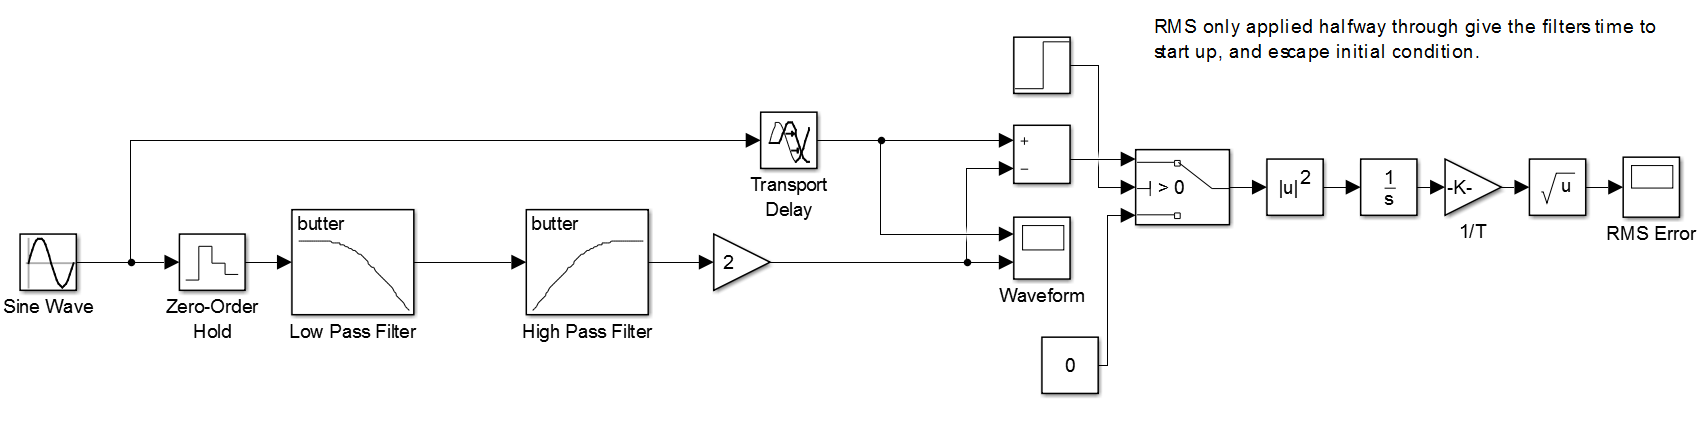
\includegraphics[width=\textwidth]{graphics/determine_max_frequency.png}
	\caption{Simulink block diagram for determining reconstructability}
	\label{fig:determine_max_frequency}
\end{figure}


A sinusoidal signal $x(t) = \sin(2\omega \pi f \cdot t)$ is discretized at interval T. 
The discrete signal is processed by a first order low pass filter, and then reconstructed by a first order highpass filter and a gain of 2.
This processed signal is then compared to the original signal delayed by $\frac{T}{2}$.
To get an estimate of the authenticity of the reconstructed signal, RMS is calculated from the difference between the delayed input signal, and the reconstructed signal.
To compare, the simulation has been performed with values of T ranging from $\frac{1}{2f}$ to $\frac{1}{10f}$.\\

%*\begin{table}[h]
%	\centering
%	\sisetup{table-space-text-post=\si{\degree}}
%	\begin{tabular}{| S | S | S |}
%		\hline
%		\rowcolor[HTML]{C0C0C0}		{T} & {$f= 333.3\si{\herz}$} & {$f= 300\si{\herz}$} \\
%		\hline
%		{$\frac{1}{2f}$} & {0.701} & {0.701} \\
%		\hline
%		{$\frac{1}{4f}$} & {0.156} & {0.15} \\
%		\hline
%		{$\frac{1}{5f}$} & {0.0983} & {0.109} \\
%		\hline
%		{$\frac{1}{6f}$} & {0.0674} & {0.0889} \\
%		\hline
%		{$\frac{1}{8f}$} & {0.0376} & {0.0744} \\
%		\hline
%		{$\frac{1}{10f}$} & {0.025} & {0.06985} \\
%		\hline
%	\end{tabular}
%	\caption{Comparison of RMS of error at maximum frequency, and 90 \%}
%	\label{tab:determine_maximum_frequency}
%\end{table}

Evidently, there are great gains to archieve by increasing the the sample rate, but this also puts extra strain on the network.
It should be mentioned, that the current measurements can be almost perfectly reconstructed by performing Clarke-Park transformation, interpolating, and then the inverse Clarke-Park transformation.
Additionally, the Matlab function, resample, produces nicely filtered vectors with smaller time steps, so it is possible to use a low sample rate for time invariant signals.\\

Another way to look at this is to calculate the maximum change in current from one sample to another.
This is determined by the inductance of the motor, which is $400 \si{\micro \henry}$, and the maximum voltage across it, which is $\frac{2}{3} V_{BAT}=35.2 \si{\volt}$. 
At a sample rate of $\frac{1}{10f}$, this results in a theoretical maximum step of $264\si{\ampere}$.
A sample rate lower than this, would make it hard to properly record such sudden steps. 
The sample rate should then be at least $\frac{1}{10f}$, which is $0.3\si{\milli \second}$.

\subsection{Data Type}
When the sample rate is known, it is possible to get an estimate of 

%Find length of strings, analog signals are 12 bits, which comes to 6 digits plus minus and comma. Time is at least 6 bytes, encoder can be as little as 2 bytes, but up to 6